\subsection{Hamming distance differential analysis}

\begin{frame}
\frametitle{Hamming distance differential analysis}
For an \textit{Encryption function }$f : f(X) \ \rightarrow \ Y$ \\
If $HD(X, \ X^\prime) \ = \ n$, then $HD(Y, \ Y^\prime) \ \stackrel{?}{=} \ m$
\setlength{\columnsep}{-30pt}
\begin{multicols}{2}
\setlength{\leftmargin}{1pt}
\begin{figure}
    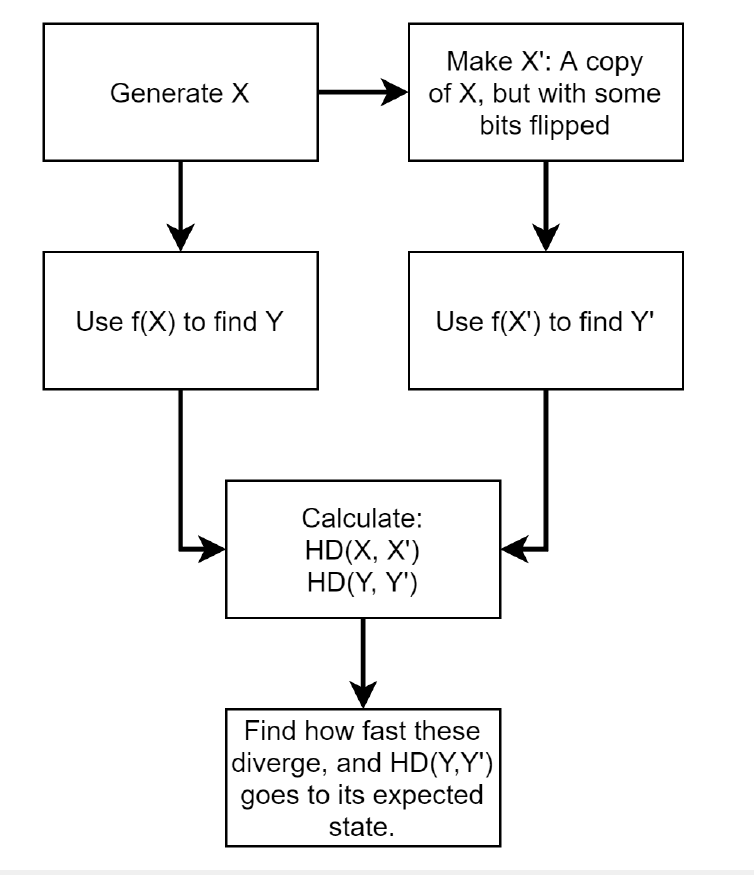
\includegraphics[scale=0.25]{HD.png}
    \tiny{\caption{Hamming Distance}}
\end{figure}
\columnbreak
\begin{itemize}
    \item If the algorithm has a good avalanche effect, we would expect the $HD$ to be about the same as the $HD$ between two random values: About half the bits.
    \item If $P$ and $Q$ are two random binary numbers of length $n$, we would expect: $HD(Q,P) \ \approx \ \dfrac{n}{2}$
\end{itemize}
\end{multicols}
\end{frame}